\chapter*{Introduction}
\label{chap:introduction}

\section{Aminoacids and proteins}

Proteins represent the last link in the central dogma of biology, where information encoded in DNA, is transcribed to RNA for posterior translation into proteins at the ribosome.

Proteins are made up of 20 basic units, called aminoacids. All aminoacids share a common chemical structure, where a carbon atom ($C_\alpha$) is covalently bonded to a hydrogen atom, a carboxyl group, an amino group, and last but not least, a radical, also called side chain of the aminoacid. The side chain differs between aminaocids and generates them from each other. A slight deviation from this pattern exists in proline, where the radical is bound to the nitrogen atom, making it an iminoacid. Even though the side chains are all different, they can be classified into four different groups: aliphatic, polar, positively charged and negatively charged (see figure \ref{fig:aminoacids}).

\begin{figure}
  \centering
  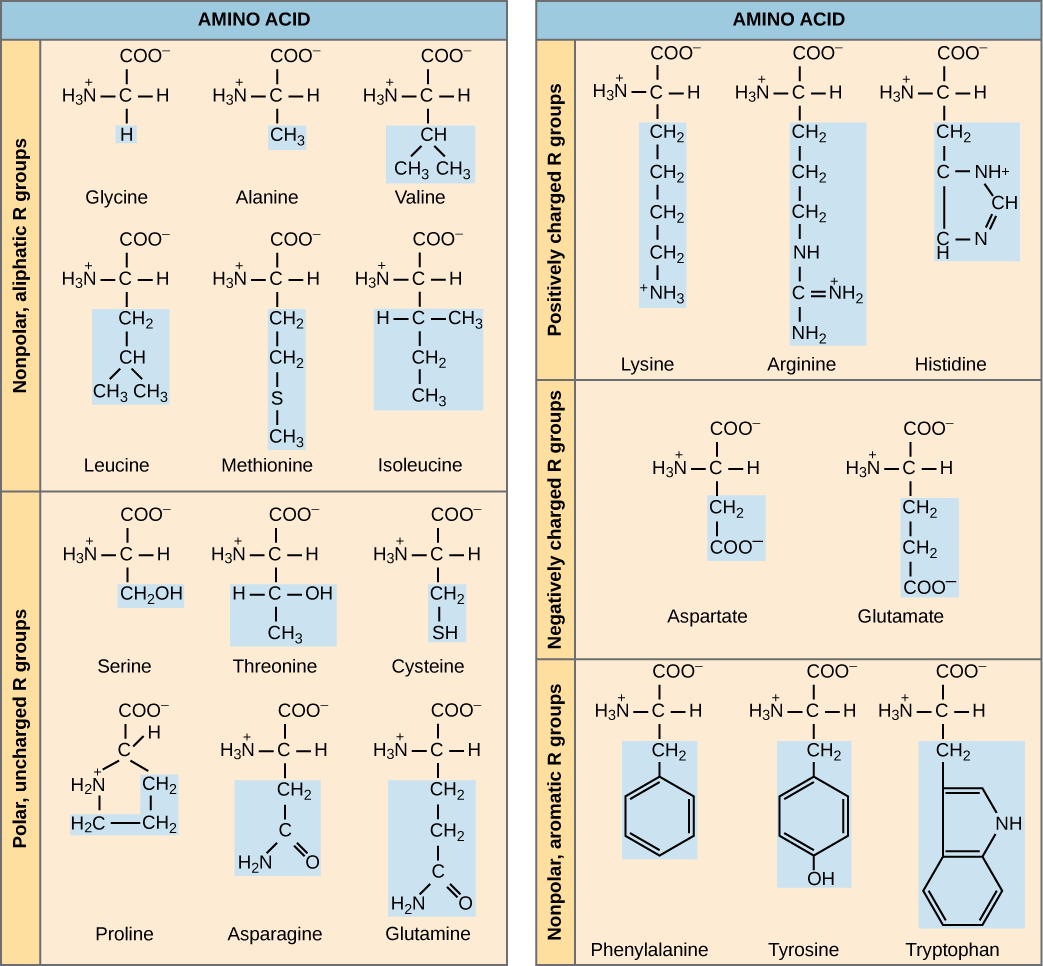
\includegraphics[width=0.8\textwidth]{aminoacids2.png}
  \caption{CAPTION AND REFERENCE}
  \label{fig:aminoacids}
\end{figure}

Two aminoacids are joined together through the formation of a peptidic (covalent) bond between them. Such a linkage is formed by removal of the elements of water (dehydration) from the $\alpha$-carboxyl group of one amino acid and the $\alpha$-amino group of another \cite{Nelson2008}. The remaining $\alpha$-amino and $\alpha$-carboxyl groups are available for linkage to other aminoacids, and in this way peptidic chains or peptides can be created.

While there are 20 basic units that constitute the majority of naturally observable proteins, their side chains can be modified both by physiological processes and by experimental procedures cite. One frequent instance of such modifications is the oxidation of methionine.


\section{The protein-focused biotechnology industry}


Proteins carry out most of the cell\textquotesingle s molecular functions, they work as molecular agents that can perform an extremely wide range of tasks. The advent of biotechnology has sought to take advantage of this power, either by using proteins as present in natural conditions (wild type) or engineered by humans. This potential economic activity is carried out by several biotech companies, including Novozymes A/S (NZ).

\ac{NZ} is a company whose line of business consists of the development of enzymatic products performing chemical transformations in different industrial processes. The application of these products, instead of conventional chemical-based solutions, has the advantage that they require less chemical substances, potentially simplifying industrial processes, reducing their costs and their environmental impact. Notorious examples of such applications include waste-water treatment, household care and the baking industry.


The advancement of the way \ac{NZ} does protein research is thus key to place the organization ahead of its competitors. The refinement of the currently used tools and the development of new ones could be of great significance for the company. 

Protein research can be approached from different angles. This thesis exploited the combination of mass spectrometry (\ac{MS}) and proteomics workflows (see chapter \ref{chap:mass_spec}) for the qualitative and quantitative characterization of protein samples.



\section{Objectives of the Thesis}
\label{sec:objectives}

In line with the goal of making \ac{NZ} more competitive, this project aimed at the following objectives:

\begin{enumerate}

\item Develop an open-source, Linux based and easily deployable pipeline for the analysis of \ac{MS} data, starting at the raw high-throughput data files and ending in the  biological interpretation of the results.

\item Evaluate this pipeline with a benchmark dataset to assess if the pipeline is able to reflect the biological phenomena captured in the data.

\item Establish a label-free quantification probabilistic model that provides relative abundance estimates and a measurement of their uncertainty based on the available data.

\end{enumerate}

\section{Structure of the Thesis}

An overview over the \ac{MS} and following computational data analysis steps is presented in \ref{chap:mass_spec}. The pipeline development and its benchmark are explained in chapters \ref{chap:pipeline} and \ref{chap:benchmark}, while the modelling problem is introduced in chapter \ref{chap:model}. Finally, a conclusion of the work is given in chapter \ref{chap:conclusion}.